\section*{Figuras (temporal)}
\begin{figure}[H]
	\centering
	
	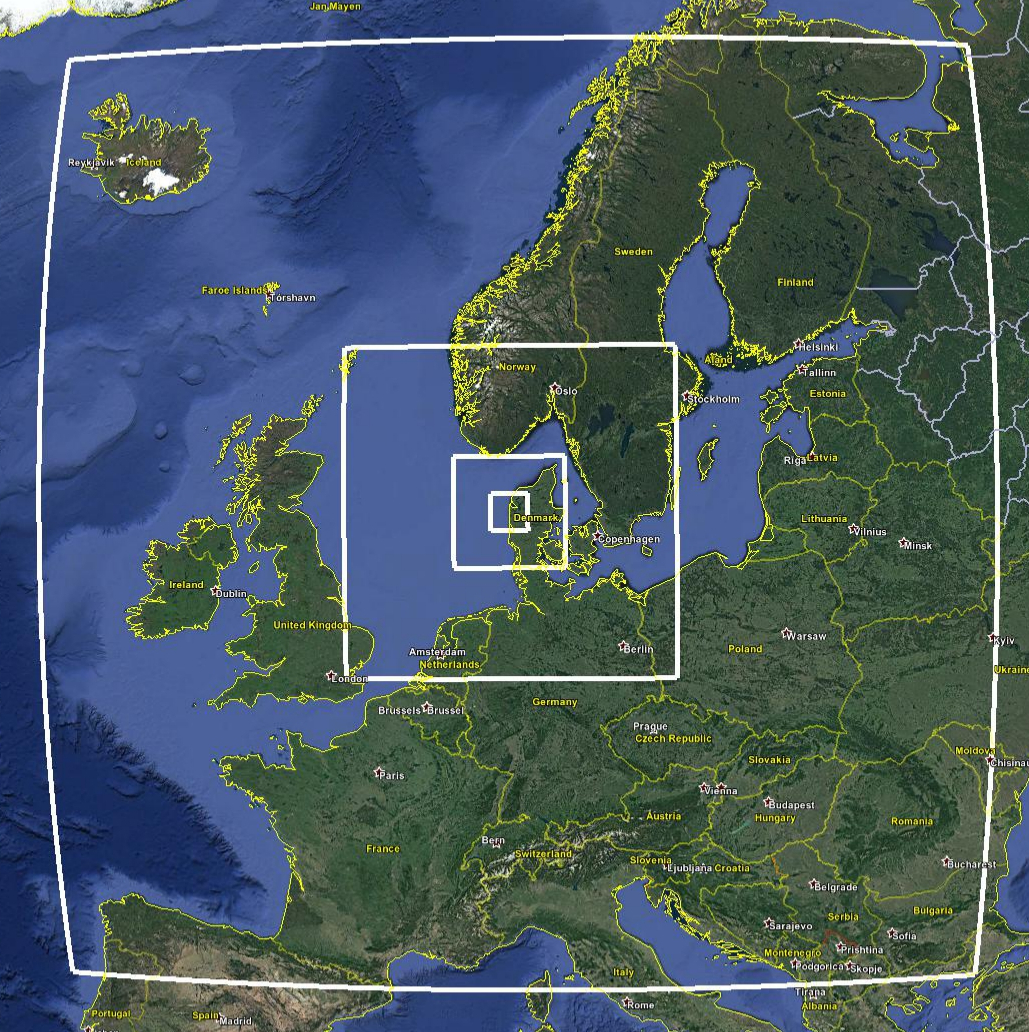
\includegraphics[height=5cm,trim={5mm 3mm 3mm 3mm},clip,frame]{Imagenes/05/hov_dom1_edit.jpg}
	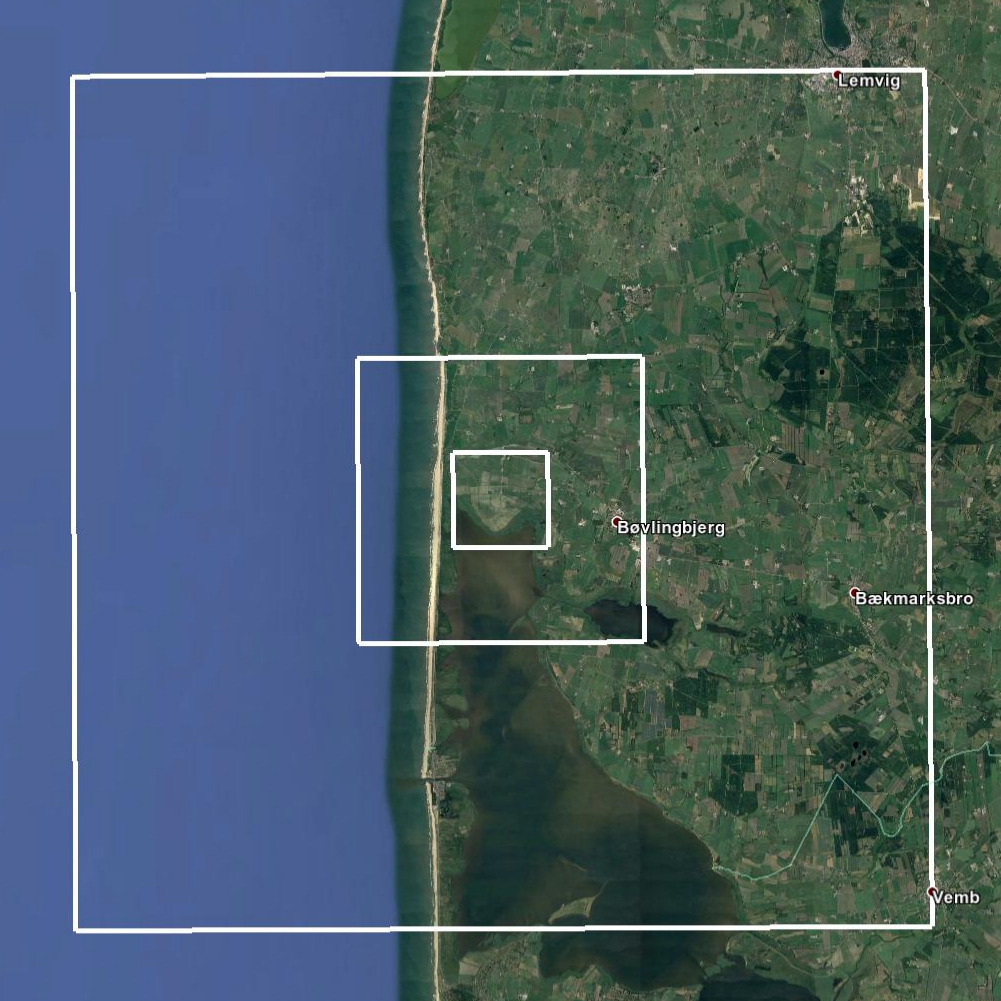
\includegraphics[height=5cm,trim={5mm 3mm 3mm 3mm},clip,frame]{Imagenes/05/hov_dom2_edit.jpg}%
	
	\caption{Simulation domains for H1 and H2. (a) Domains d1-d4. (b) d5-d7.}
	\label{fig:05_dom_hov}
\end{figure}

%\begin{figure}[H]
%	\centering
%	\includegraphics[height=5cm,page=1,trim={5mm 3mm 3mm 3mm},clip,frame]{Imagenes/05/bol_d1-2-3-4edit.jpg}
%	\includegraphics[height=5cm,page=1,trim={5mm 3mm 3mm 3mm},clip,frame]{Imagenes/05/bol_d4-5-6edit.jpg}
%	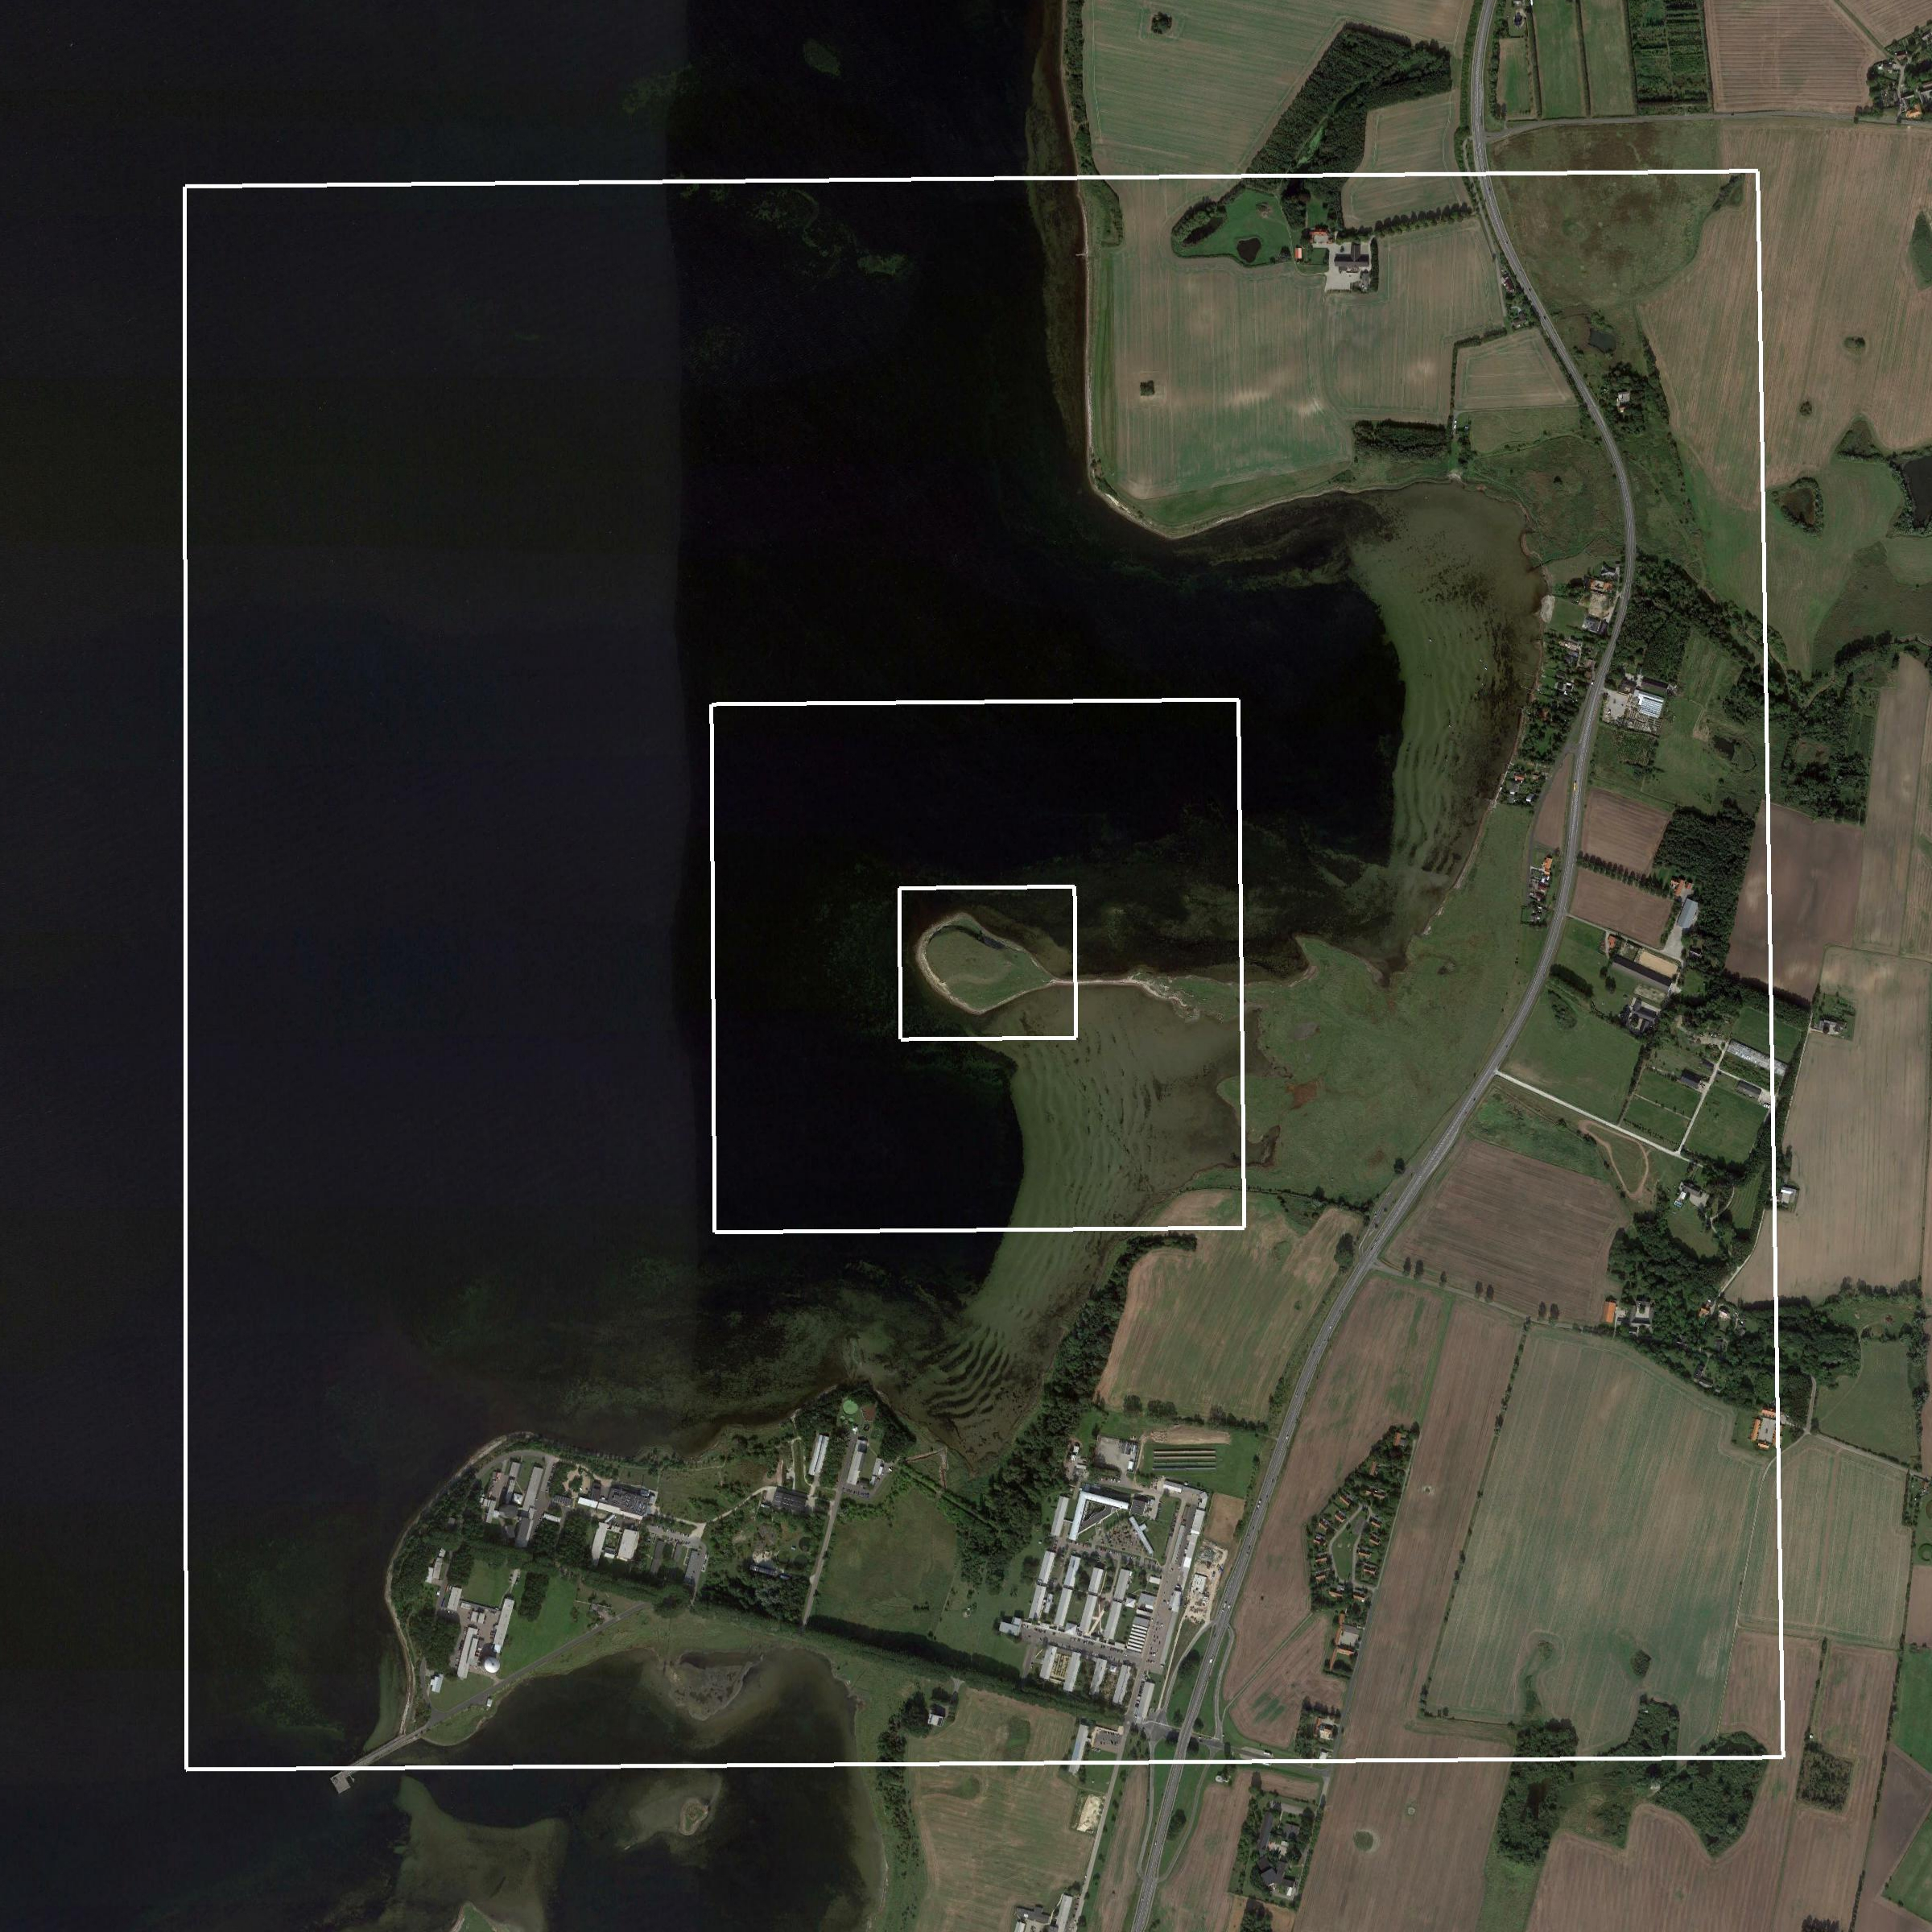
\includegraphics[height=5cm,page=1,trim={5mm 3mm 3mm 3mm},clip,frame]{Imagenes/05/bol_d6-7-8edit.jpg}%
%	
%	\caption{Simulation domains for B1, B2 and B3. (a) d1-d4. (b) d4-d6. (c) d6-d8.}
%	\label{fig:05_dom_bol}
%\end{figure}

\begin{figure}[H]
	\centering
	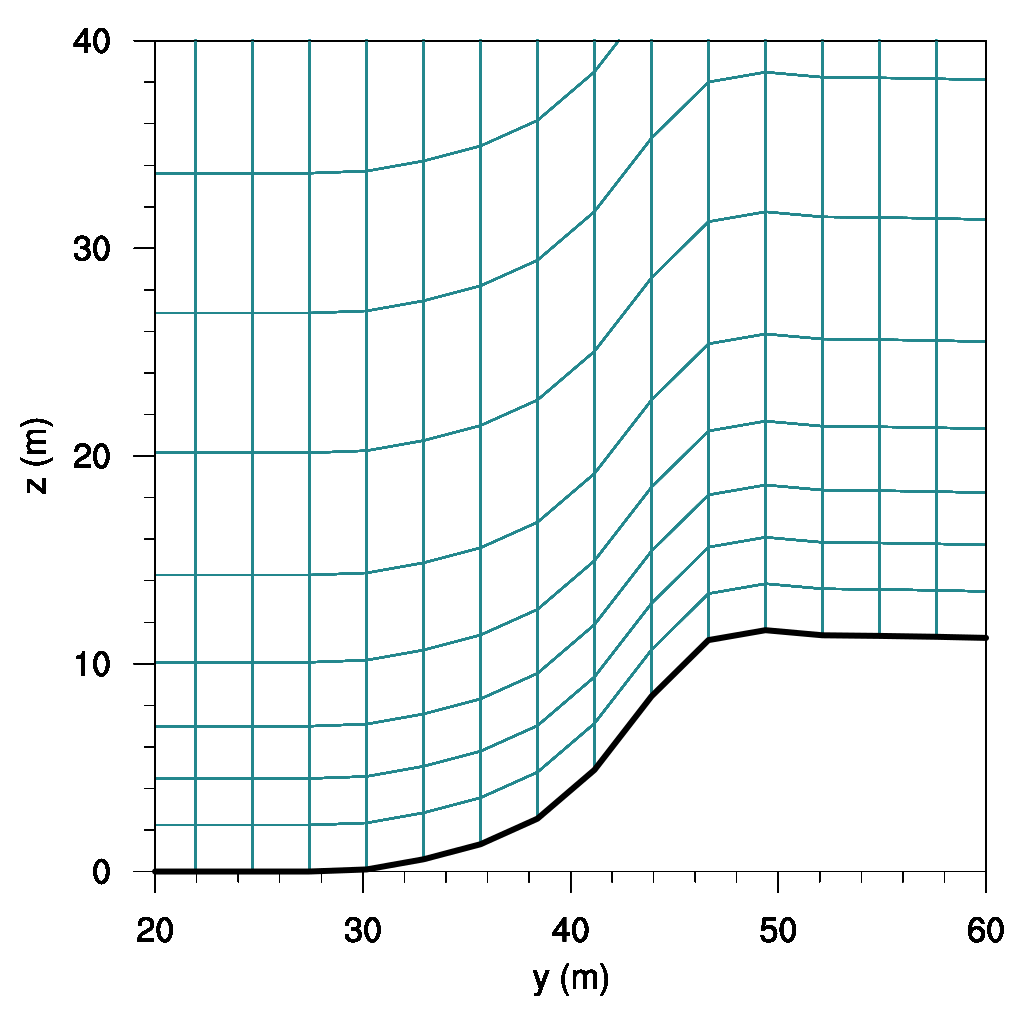
\includegraphics[height=5cm,trim={0cm 0cm 0cm 0cm},clip]{Imagenes/05/hd_mesh_50}
	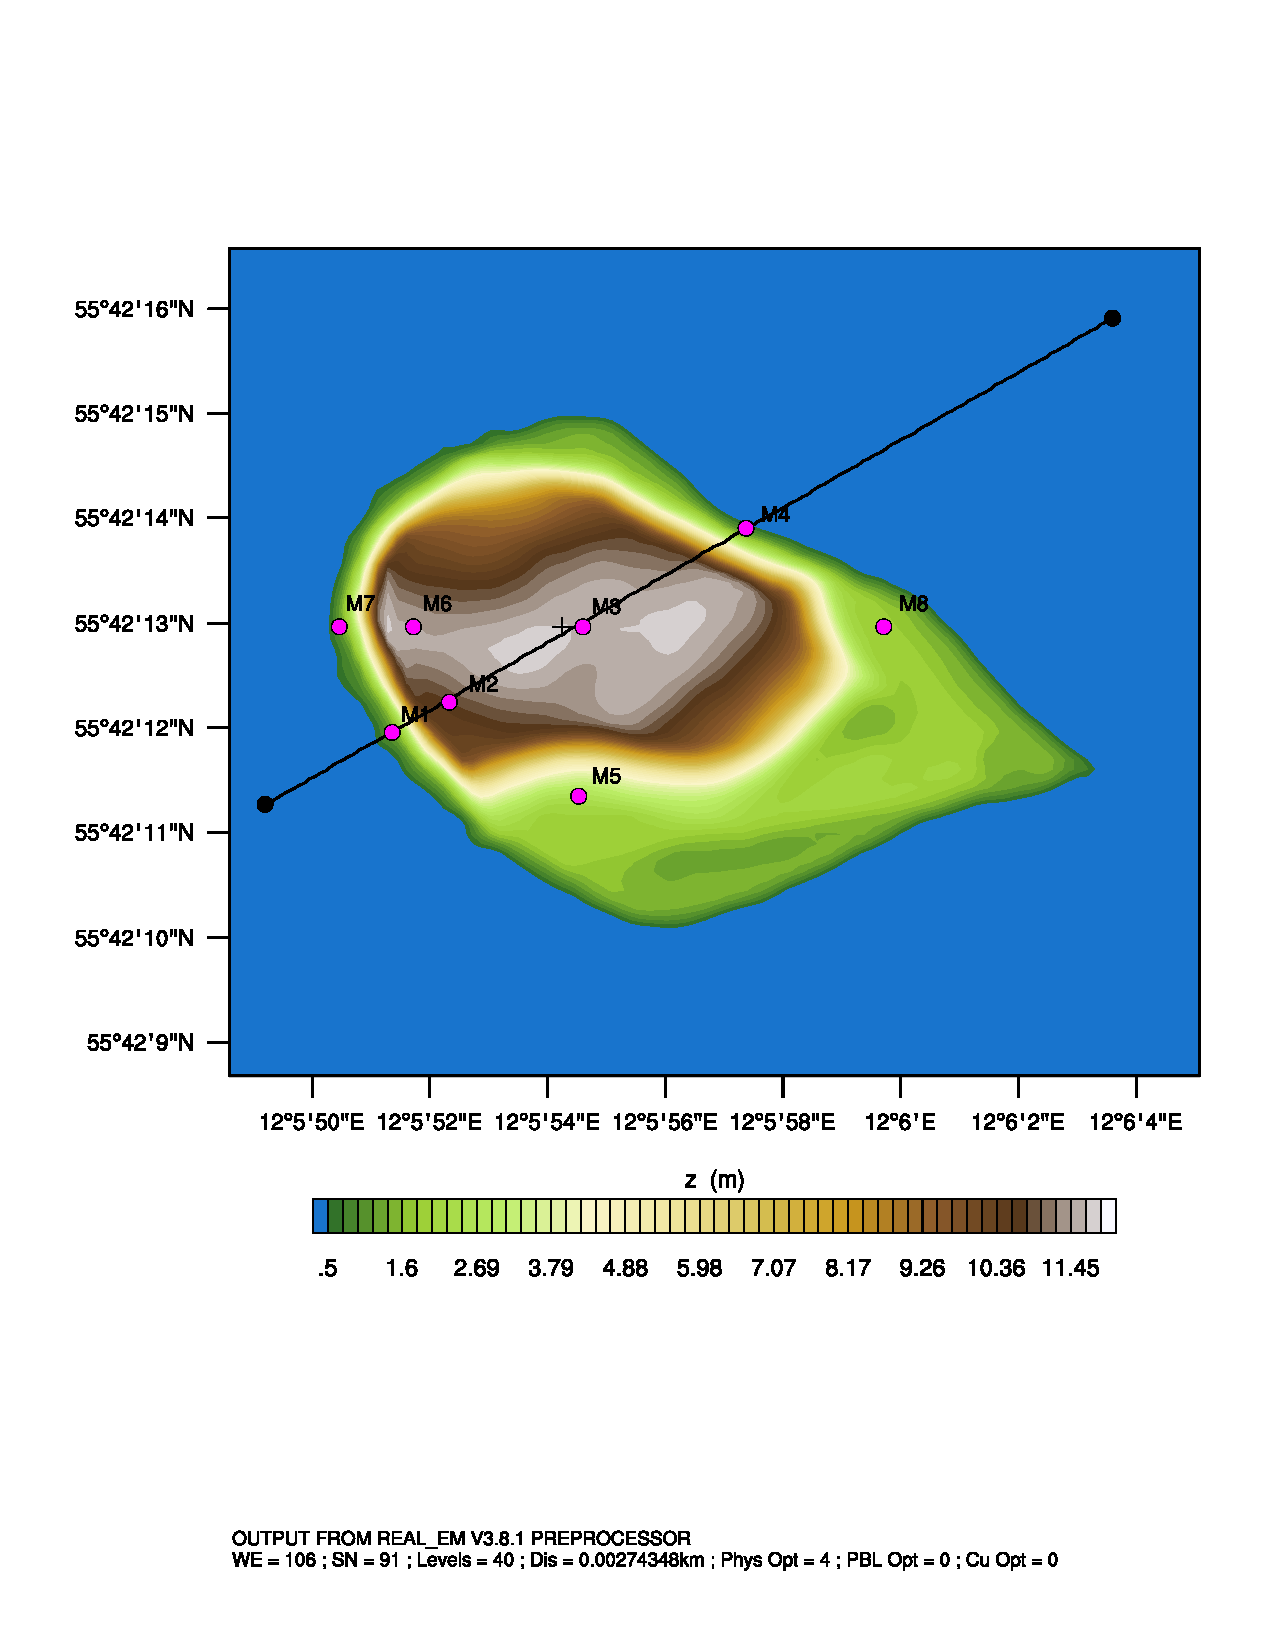
\includegraphics[height=5cm,page=1,trim={3.4cm 9.3cm 1cm 4cm},clip]{Imagenes/05/bol_control_point.pdf}%
	
	\caption{(a) Detail the steep slope on a 1:1 scale. (b) Control points locations for B1, B2 and B3. }
	\label{fig:05_mesh_bol}
\end{figure}

\begin{figure}[H]
	\centering
		\includegraphics[height=0.62\linewidth,page=37,trim={35mm 10mm 41mm 25mm},clip]{Imagenes/06/hov/9u}%
		\includegraphics[height=0.62\linewidth,page=37,trim={48mm 10mm 41mm 25mm},clip]{Imagenes/06/hov/9v}%
		\includegraphics[height=0.62\linewidth,page=37,trim={48mm 10mm 41mm 25mm},clip]{Imagenes/06/hov/9V}%

	\caption{Comparación de la simulación (línea continua) con la simulación de Peña et. al. en el 2013 (línea punteada) y valores medidos para (a) componente $u$ de la velocidad del viento, (b) componente $v$ y (c) magnitud de la velocidad del viento. Los datos corresponden a promedios temporales entre las 12:00 y 15:00, y han sido rotados de tal forma que su dirección sea 0$^\circ$ a los 10m.}
	\label{fig:06_hov_pena}
\end{figure}

\begin{figure}[H]
	\centering
	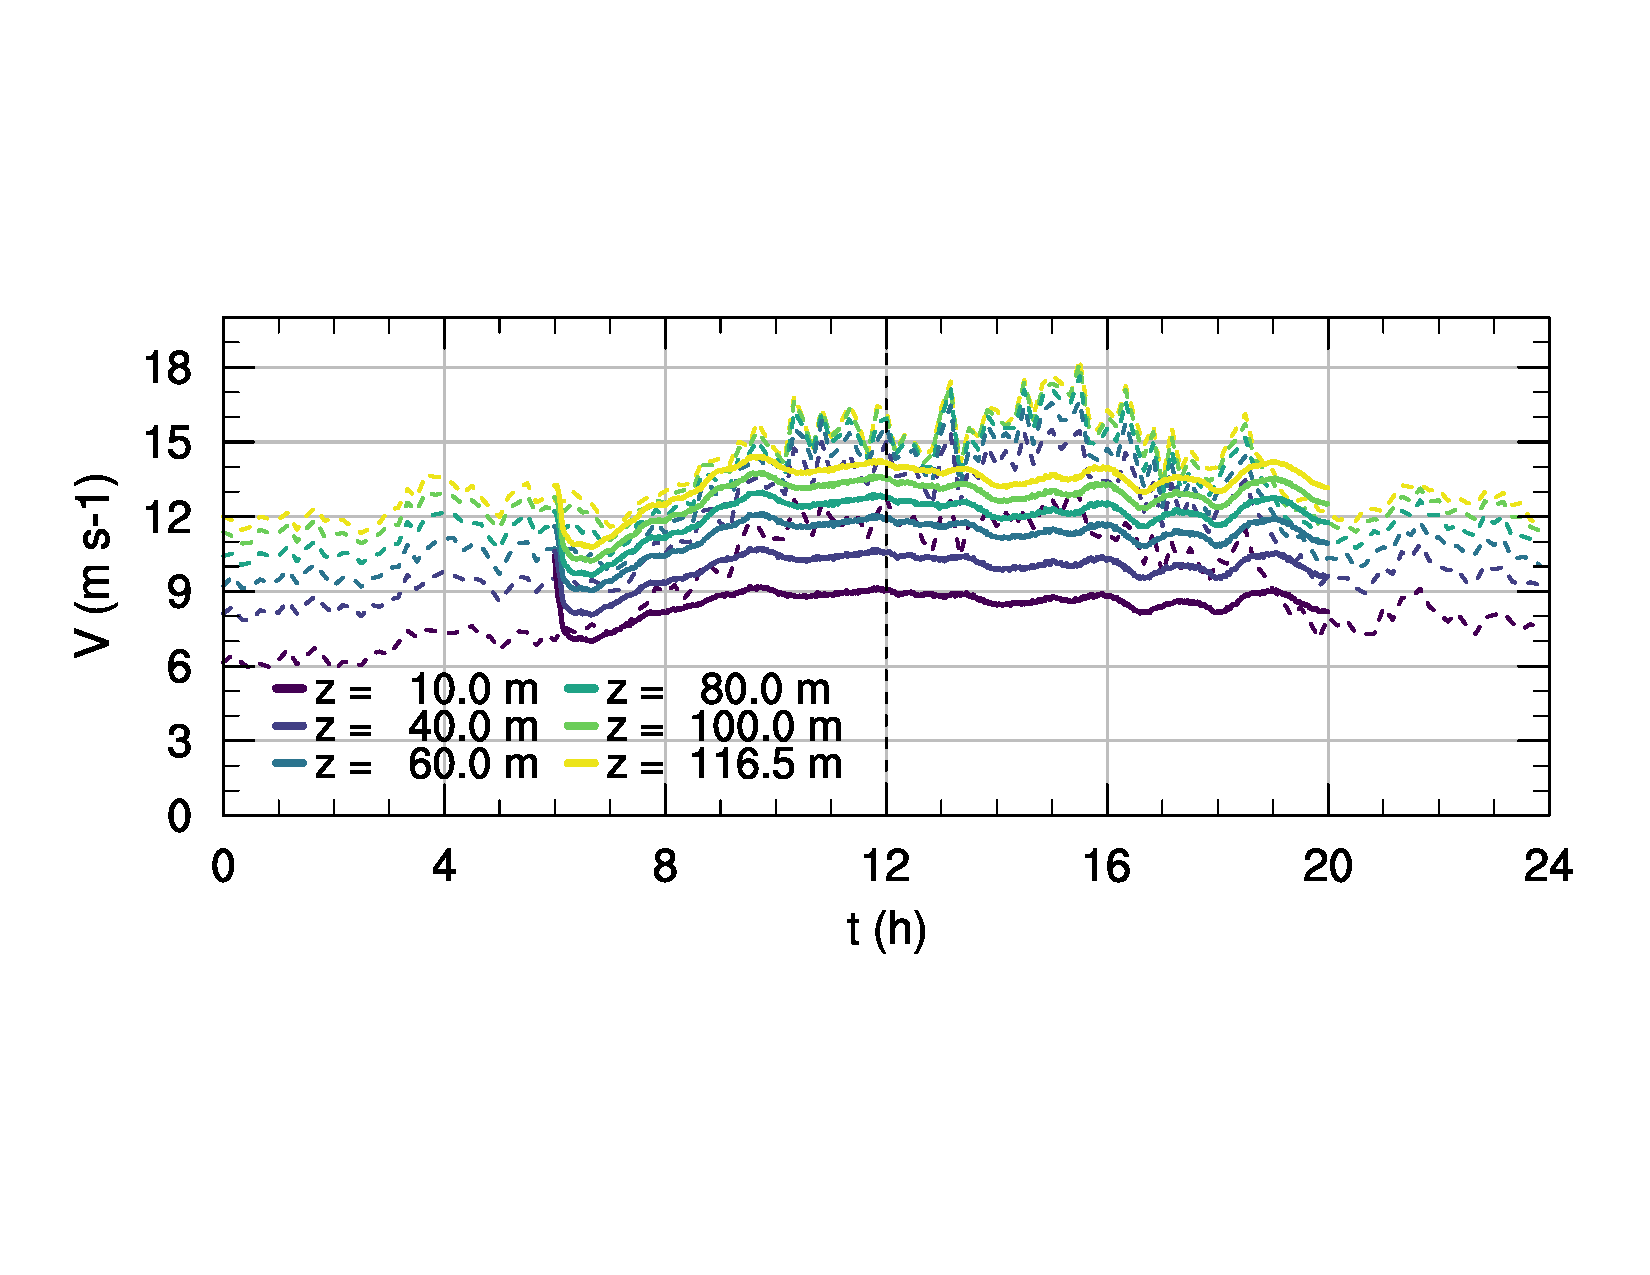
\includegraphics[width=0.5\linewidth,trim={9mm 63mm 10mm 55mm},clip]{Imagenes/06/hov/ts_v}%
	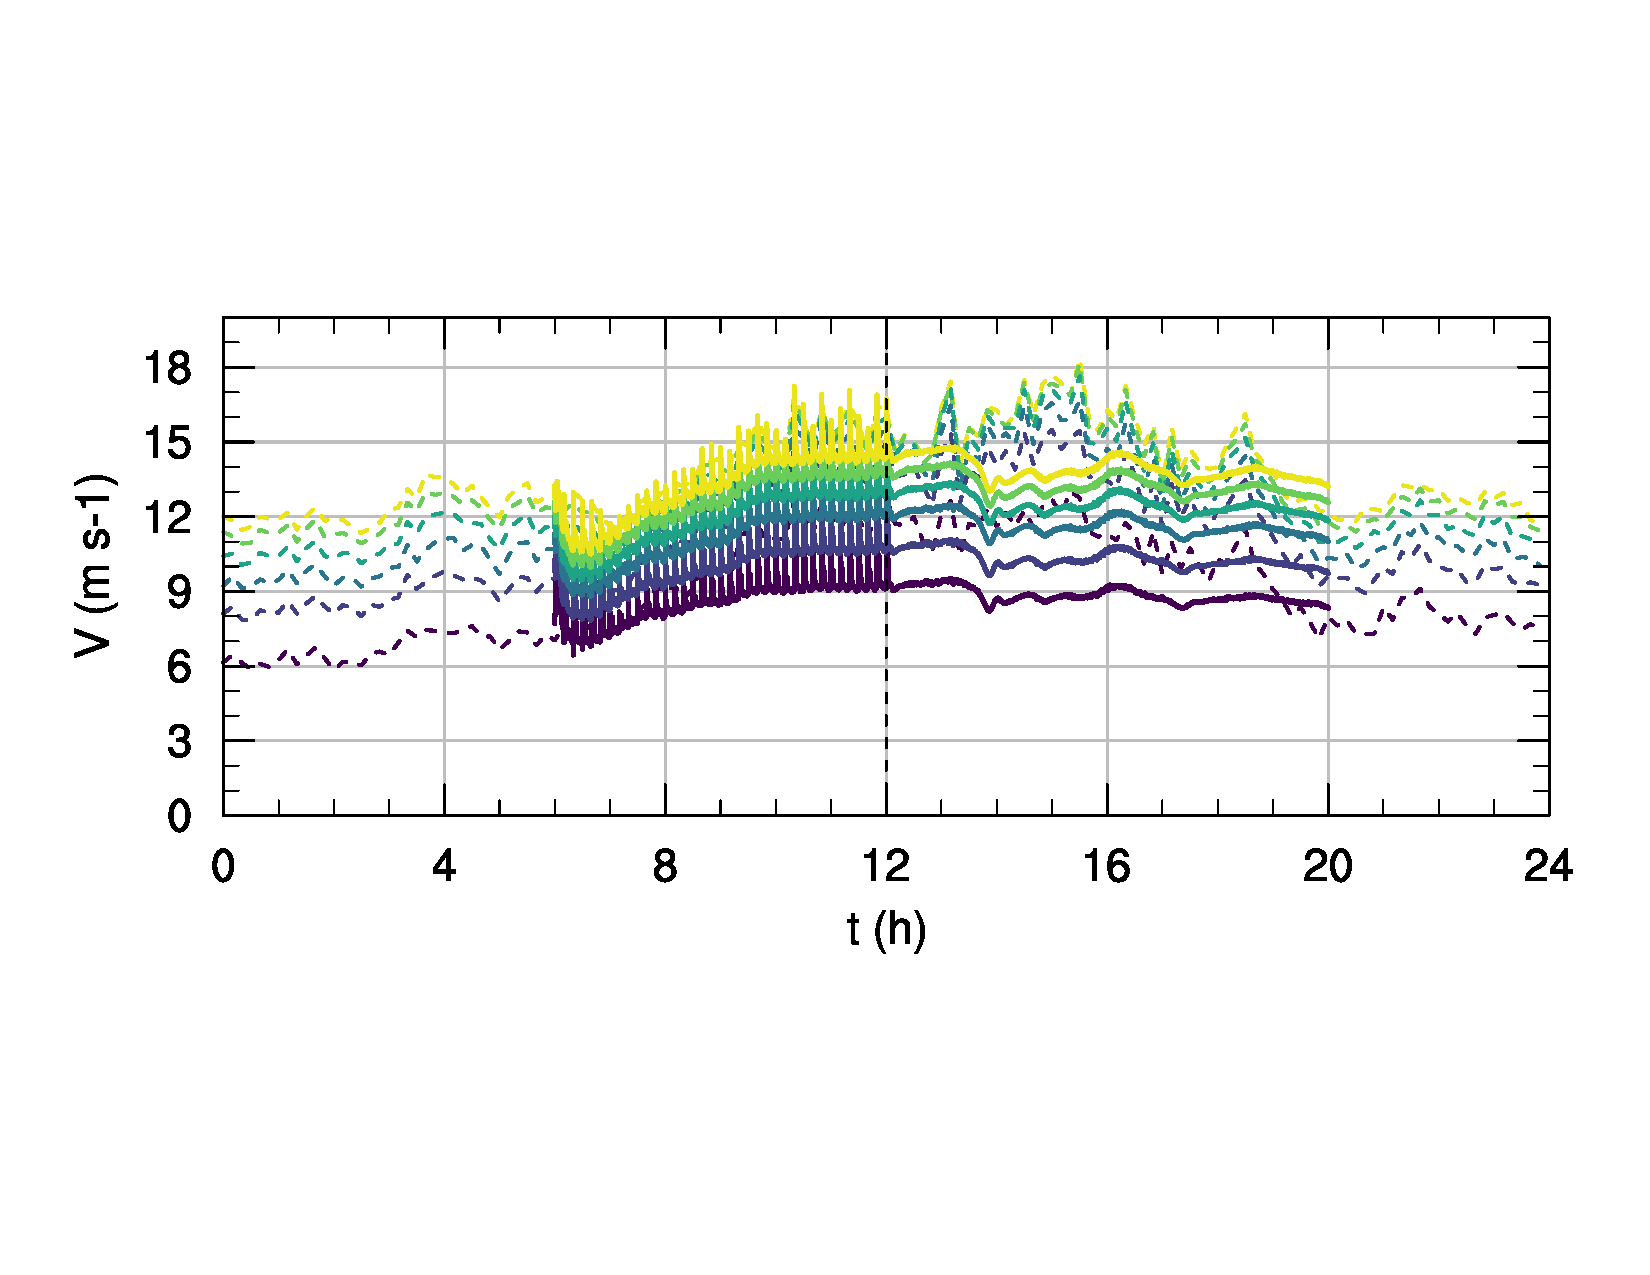
\includegraphics[width=0.5\linewidth,trim={9mm 63mm 10mm 55mm},clip]{Imagenes/06/hov_da/ts_v}%
	
	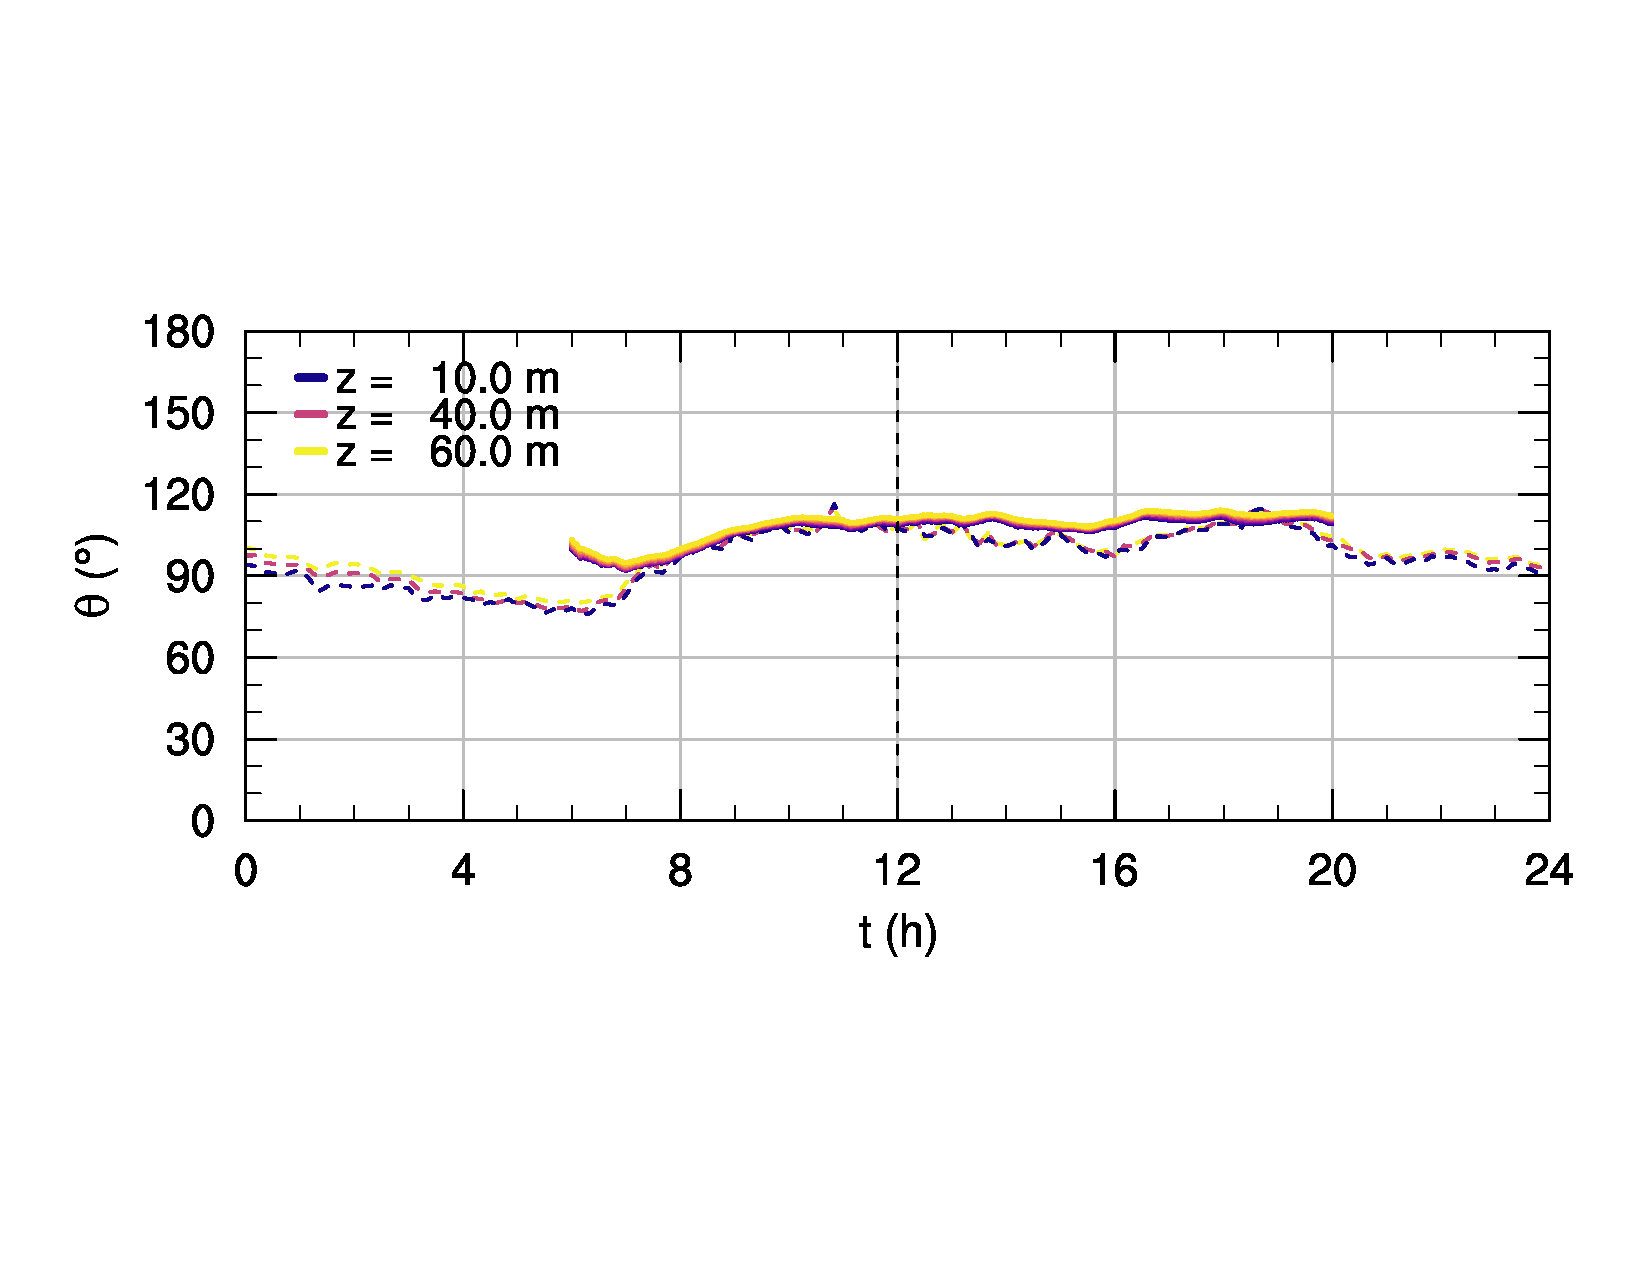
\includegraphics[width=0.5\linewidth,trim={12mm 55mm 10mm 55mm},clip]{Imagenes/06/hov/ts_o}%
	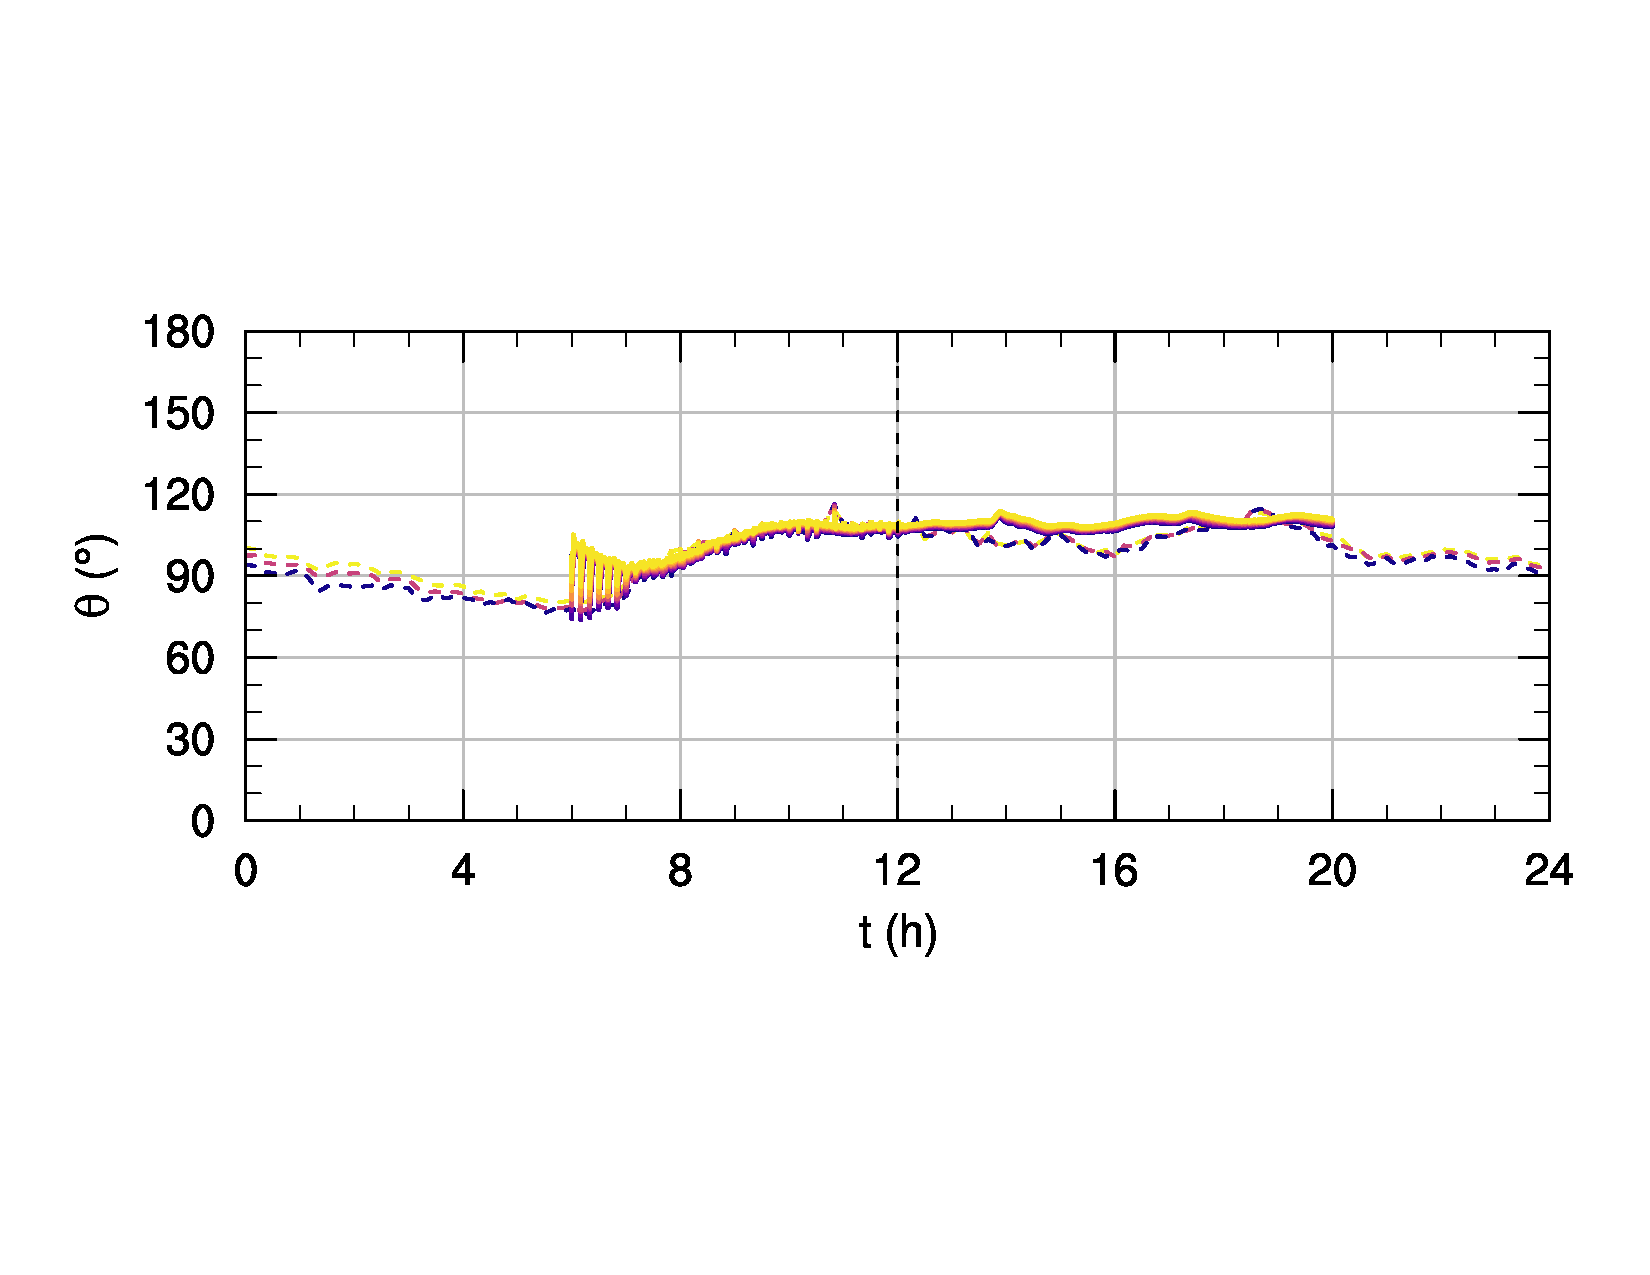
\includegraphics[width=0.5\linewidth,trim={12mm 55mm 10mm 55mm},clip]{Imagenes/06/hov_da/ts_o}%
	\caption{aaaaa}
	%\caption{Serie de tiempo para la rapidez instantánea del viento $V$ y su dirección en la ubicación del mástil meteorológico. La línea continua corresponde a lo datos simulados interpolados a las alturas de medición (solo para $V$) y la línea punteada a los datos medidos en el mástil.}
	\label{fig:06_hov_ts}
\end{figure}

\begin{figure}[H]
	\centering
	\includegraphics[width=0.9\linewidth,trim={12mm 84mm 10mm 74mm},page=37,clip]{Imagenes/06/bol/speedup}\\%
	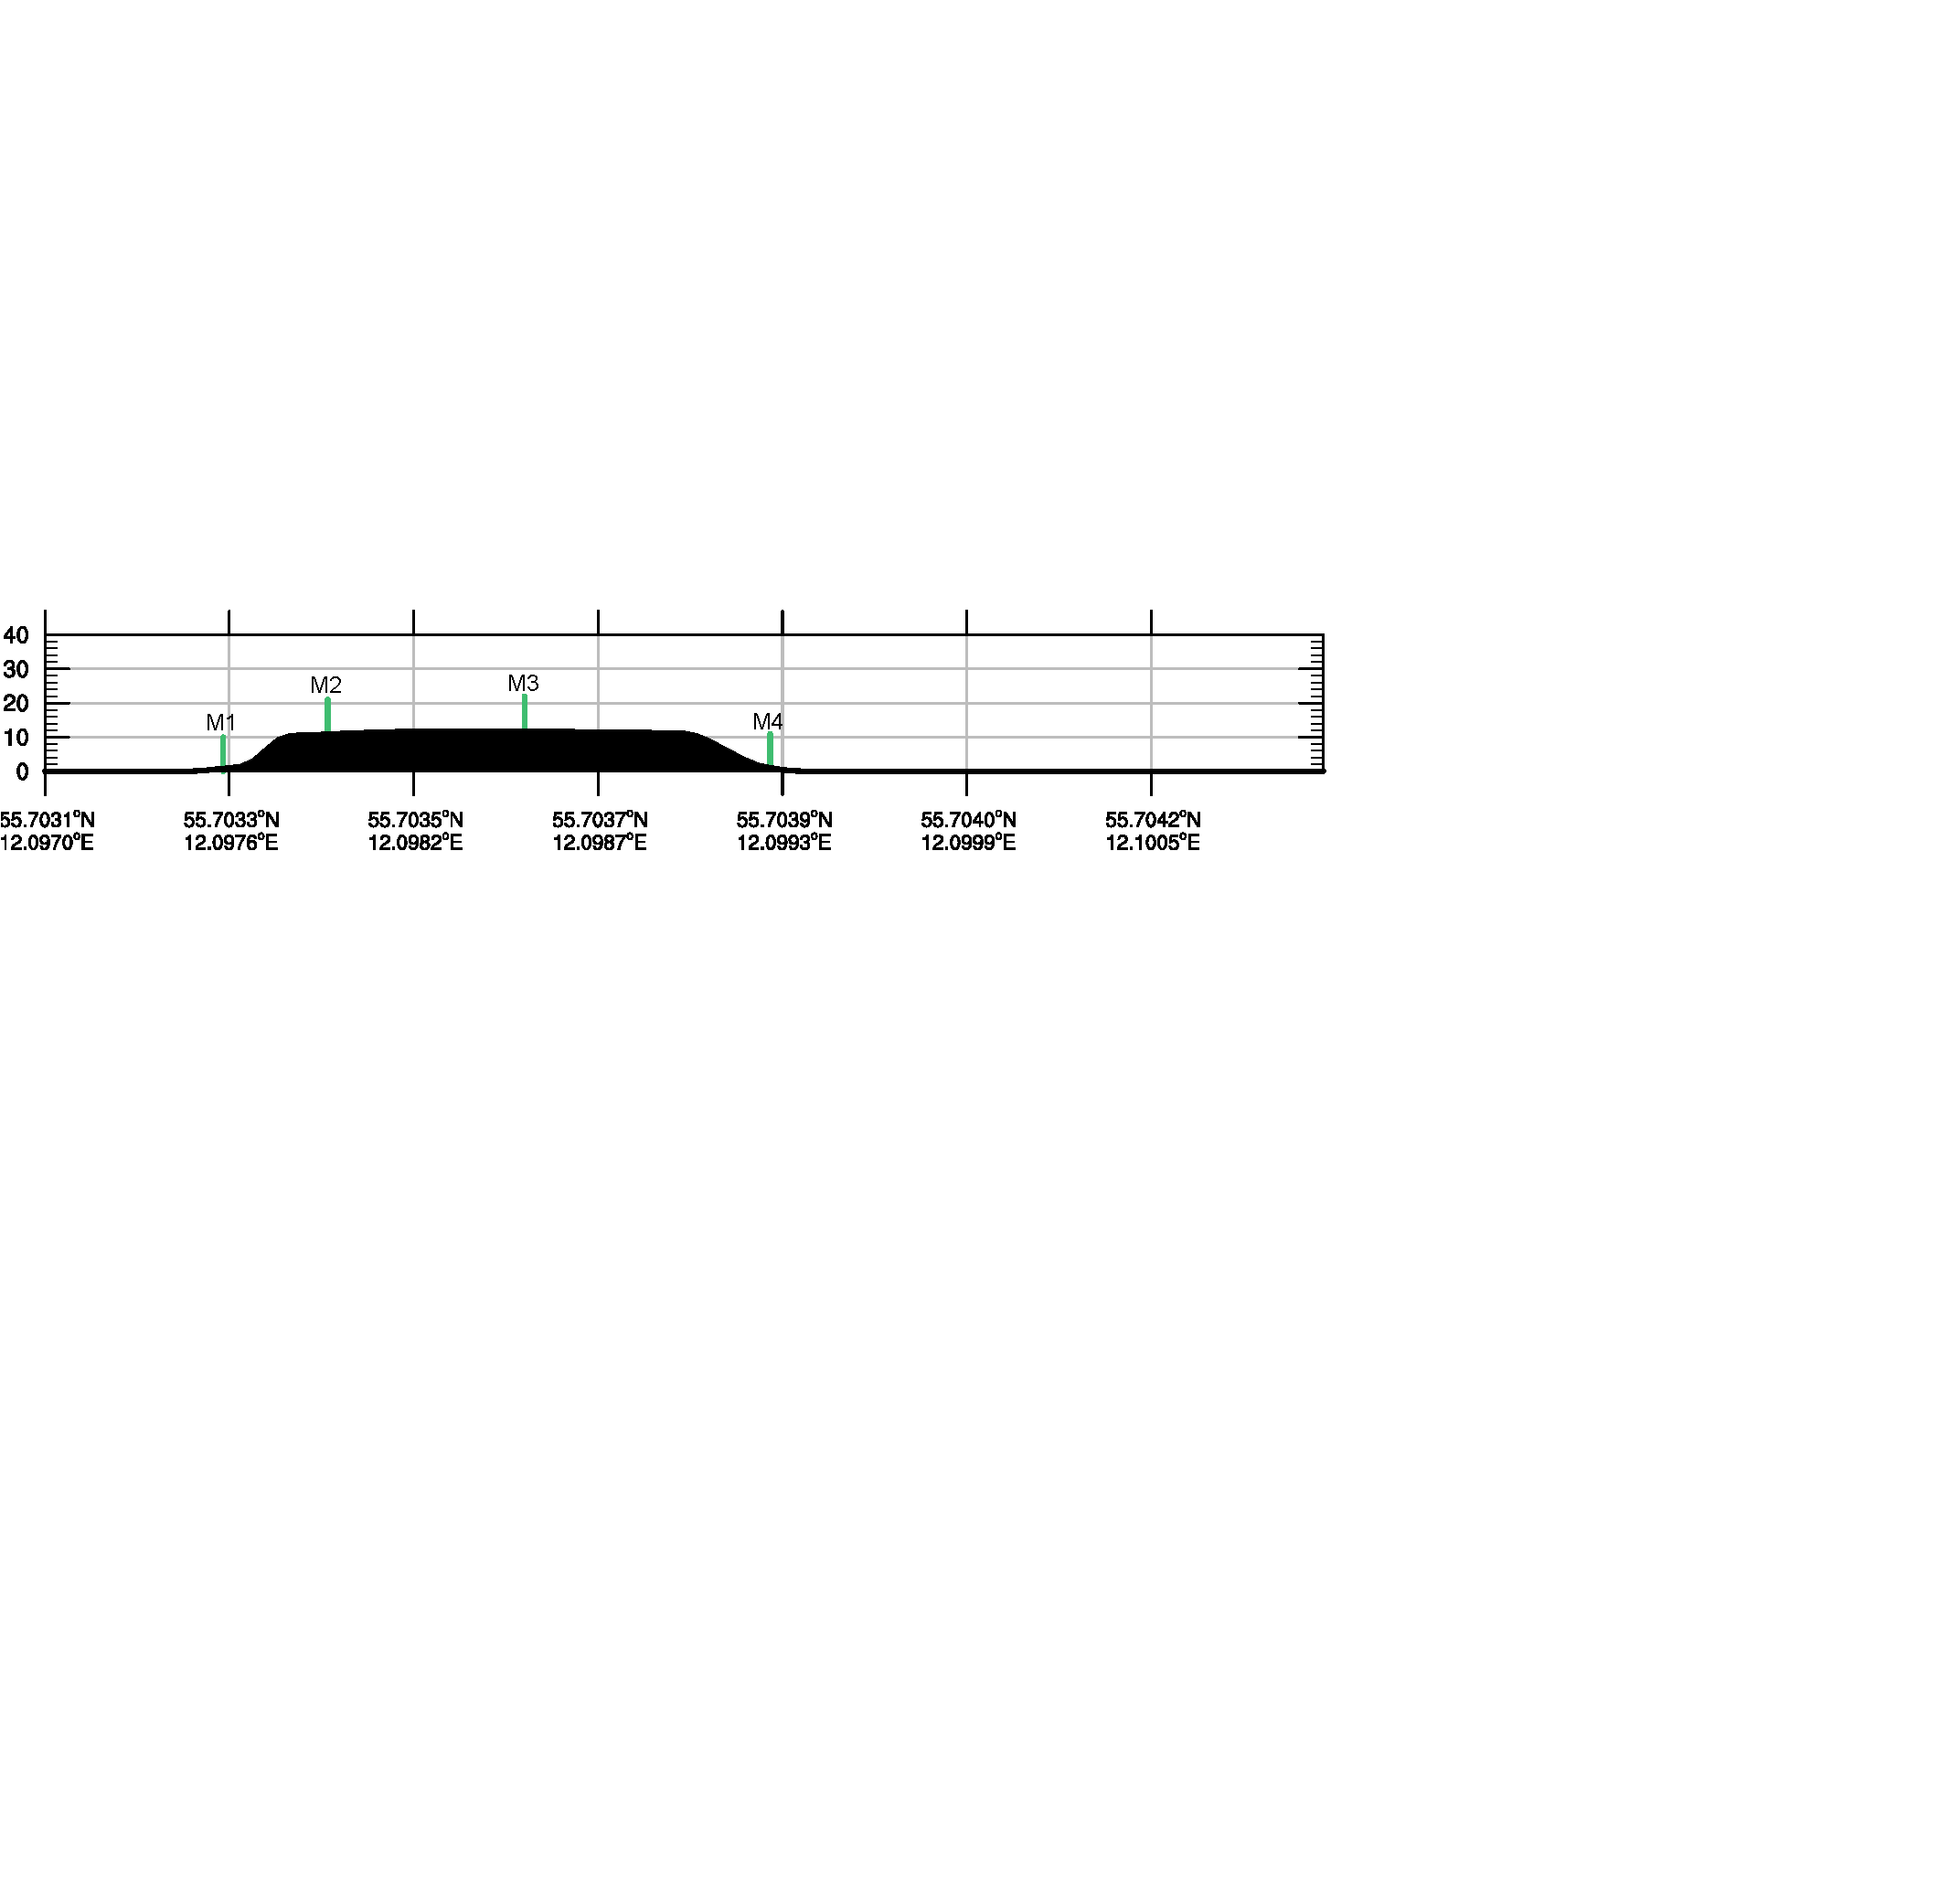
\includegraphics[width=0.9\linewidth,trim={-11mm 205mm 115mm 112mm},clip]{Imagenes/06/bol/cross_height}\\%
	\caption{Speedup en los primeros 3 niveles del modelo ($1.1$ [m] azul; $3.4$ [m] verde; $5.6$ [m] amarillo) para la sección de corte a 240$^\circ$ en Bolund. Se muestran los resultados para las 15:00 horas.}
	\label{fig:06_bol_speedup}
\end{figure}

\begin{figure}[H]
	\centering
	\includegraphics[width=0.5\linewidth,page=4,trim={9mm 57mm 10mm 60mm},clip]{Imagenes/06/bol/ts_interpol_compare.pdf}%
	\includegraphics[width=0.5\linewidth,page=4,trim={9mm 57mm 10mm 60mm},clip]{Imagenes/06/bol_da/ts_interpol_compare.pdf}%
	
	\includegraphics[width=0.5\linewidth,page=4,trim={12mm 52mm 10mm 60mm},clip]{Imagenes/06/bol/ts_interpol_compare_o.pdf}%
	\includegraphics[width=0.5\linewidth,page=4,trim={12mm 52mm 10mm 60mm},clip]{Imagenes/06/bol_da/ts_interpol_compare_o.pdf}%
	\caption{aaaaa}
	\label{fig:06_bol_ts_m4}
\end{figure}


\begin{table}[h!]
	\caption{Comparación de métricas para el caso II Bolund.}
	\label{tab:06_bol_mae_rmse}
	\centering%\footnotesize
	\begin{tabular}{lcc}
		\toprule
		& Sin DA & Con DA \\
		\midrule
		MAE & 2.6724 m/s & 4.3562 m/s \\
		RMSE & 2.9538 m/s& 4.90071 m/s\\
		$\Delta{RMSE}$&  -- & $-65.91\%$ \\
		$\Delta{MAE}$ &  -- & $-63.01\%$ \\
		\bottomrule
	\end{tabular}
\end{table}
\begin{table}[H]
	\caption{Comparación de métricas para el caso I Høvsøre.}
	\label{tab:06_hov_mae_rmse}
	\centering%\footnotesize
	\begin{tabular}{lcc}
		\toprule
		& Sin DA & Con DA \\
		\midrule
		MAE & 2.41091 m/s & 2.16742 m/s \\
		RMSE & 2.80142 m/s& 2.55778 m/s\\
		$\Delta{RMSE}$& --  & $8.70\%$  \\
		$\Delta{MAE}$ & -- & $10.47\%$  \\
		\bottomrule
	\end{tabular}
\end{table}